Nalu supports two discretizations: control volume finite element
and (CVFEM) edge-based vertex centered (EBVC). Each are finite volume forumations
and each solve for the primitives are are each considered vertex-based
schemes. Considerable testing has provided a set of general rules as to which
scheme is optimal. In general, all equations and boundary conditions
support either equation discretization with exception of the solid stress equation
which has only been implemented for the CVFEM technique.

For generalized unstructured meshes that have poor quality,
CVFEM has been shown to excell in accuracy and robustness. This is mostly
due to the inhearant accuracy limitation for the non-orthogonal
correction terms that appear in the diffusion term and pressure
stabilization for the EBVC scheme. For generalized unstructured meshes of decent quality, either 
scheme is ideal. Finally, for highly structured meshes with substantail aspect 
ratios, the edge-based scheme is ideal.

In general, the edge-based scheme is at least two times faster per iteration 
than the element-based scheme. For some classes of flows, it can be up
to four times faster. However, due to the lagged coupling between the projected
nodal gradient equation and the dofs, on meshes with high non-orthogonality,
nonlinear residual convergence can be delayed.

\subsection{CVFEM Dual Mesh}

The classic low Mach algorithm uses the finite volume technique known
as the control volume finite element method, see Schneider,~\cite{Schneider:1987}, or 
Domino,~\cite{Domino:2006}. Control volumes 
(the mesh dual) are constructed about the nodes, shown in Figure~\ref{hoCVFEM} (upper left).
Each element contains a set of sub-faces that define control-volume surfaces.
The sub-faces consist of line segments (2D) or surfaces (3D).
The 2D segments are connected between the element centroid
and the edge centroids. The 3D surfaces (not shown here) are connected between
the element centroid, the element face centroids, and the
edge centroids. Integration points also exist within the sub-control
volume centroids. 

Recent work by Domino,~\cite{Domino:2014}, has provided a proof-of-concept higher order CVFEM implementation 
whereby the linear basis and dual mesh definition is extended to higher order. The curent code base supports
the usage of P=2 elements (quadratic) for both 2D and 3D quad/hex topologies. This method has been formally 
demonstrated to be third-order spatially accurate and second-order in-time accurate. General polynomial promotion
has been deployed in the higher order github branch. Figure~\ref{hoCVFEM} illustrates a general polynomial promotion
from P=1 to P=6 (left) and demonstrated spectral convergence using the method of manufactured solutions (right).

\begin{figure}[h!tp]
\centering
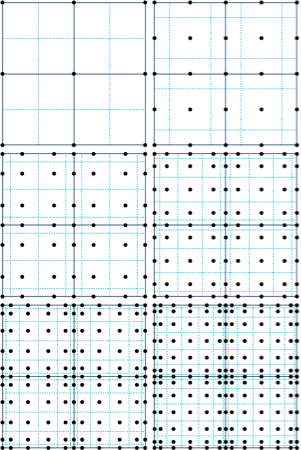
\includegraphics[clip,width=0.3\textwidth]{images/cvfem_nodes.png}
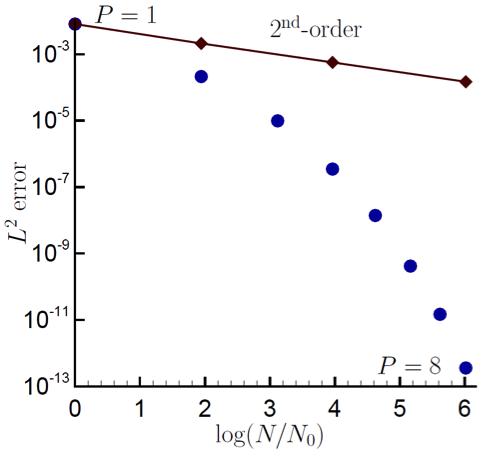
\includegraphics[clip,width=0.4\textwidth]{images/cvfem_conv.png}
\caption{Polynomial promotion for a canonical CVFEM quad element patch from $P=1$ to $P=6$ (left) and a recent spectral convergence plot using the 
Method of Manufactured Solutions for $P=1$ through $P=8$ (right).}
\label{hoCVFEM}
\end{figure}

When using CVFEM, the discretized equations described in this manual
are evaluated at either subcontrol-surface integration points (terms that
have been integrated by parts) or at the subcontrol volume (time and
source terms). Interpolation within the element is obtained by the
standard elemental basis functions,

\begin{equation}
\phi_{ip} = \sum N^{ip}_k \phi_k.
\label{cvfemInterpolation}
\end{equation}
%
where the index $k$ represents a loop over all nodes in the element.

Gradients at the subcontrol volume surfaces are obtained by taking the derivative
of Eq.~\ref{cvfemInterpolation}, to obtain,

\begin{equation}
\frac{\partial \phi_{ip}}{\partial x_j} = \sum \frac{\partial N^{ip}_{j,k}} {\partial x_j} \phi_k.
\label{cvfemDerivative}
\end{equation}

The usage of the CVFEM methods results in the canonical 27-point stencil
for a structured hexahedral mesh.

\subsection{Edge-Based Discretization}
In the edge-based discretization, the dual mesh defined in the CVFEM
method is used to pre-process both dual mesh nodal volumes (needed in
source and time terms) and edge-based area vectors (required for integrated-by-parts
quantities, e.g., advection and diffusion terms).

Consider Figure~\ref{hoCVFEM}, which is the original set of CVFEM
dual mesh quadrature points shown above. Specifically, there are four subcontrol
volumes about node 5 that contribute to the nodal volume dual mesh.
In an edge-based scheme, the time and source terms use single point
quadrature by assembling these four subcontrol volume contributions
(eight in 3D) into one single nodal volume. In most cases, source terms
may include gradients that are obtained by using the larger element-based
stencil.

The same reduction of gauss points is realized for the area vector.
Consider the edge between nodes 5 and 6. In the full CVFEM approach,
subcontrol surfaces within the top element (5,6,9,8) and bottom
element (2,3,6,5) are reduced to a single area vector at the 
edge midpoint of nodes 5 and 6. Therefore, advection and diffusion
is now done in a manner very consistent with a cell centered scheme, i.e.,
classic ``left''/''right'' states.

The consolidation of time and source terms to nodal locations along with
advection and diffusion at the edge mid-point results in a canonical
five-point stencil in 2D and seven in 3D. Note the ability to handle
hybrid meshes is readily peformed one nodal volume and edge area are
pre-processed. Edges and nodes are the sole topology that are iterated,
thus making this scheme highly efficient, although inherantly limited to 
second order spatial order of accuracy.

In general, the edge-based scheme is second order spatially accurate.
Formal verification has been done to evaluate the accuracy of the EBVC
relative to other implemented methods (Domino,~\cite{Domino:2014}). The edge-based scheme,
which is based on dual mesh post-processing, represents a commonly used finite volume 
method in gas dynamics applications. The method also lends itself to psuedo-higher order 
methodologies by the blending of extrapolated values using the projected nodal 
gradient and gauss point values (as does CVFEM). This provides a fourth order
accurate diffusion and advection operator on a structured mesh.

The use of a consistent mass matrix is less apparent in edge-based
schemes. However, if desired, the full element-based stencil can
be used by iterating elements and assembling to the nodes. 

The advantage of edge-based schemes over cell centered schemes is
that the scheme naturally allows for a mixed elemental discretization. Projected nodal gradients
can be element- or edge-based.  LES
filters and nodal gradients can also exploit the inherant elemental
basis that exists in the pure CVFEM approach. In our experience, the optimal scheme on high quality
meshes uses the CVFEM for the continuity solve and EBVC discretization for all other equations.
This combination allows for the full CVFEM diffusion operator for the pressure Poisson equation
and the EBVC approach for equations where inverse Reynolds scaling reduces the importance of the 
diffusion operator. This scheme can be activated by the use of the ``$use \textunderscore edges: yes$''
Realm line command in combination of the LowMachEOM system line command, 
``$element \textunderscore continuity \textunderscore eqs : yes$''.

\subsection{Projected Nodal Gradients}
In the edge or element-based algorithm, projected nodal gradients
are commonplace. Projected nodal gradients are used in the fourth 
order pressure stabilization terms, higher order upwind methods, discontinuity
capturing operators (DCO) and turbulence source terms. For an edge-based scheme, 
they are also used in the diffusion term when non-orthogonality of the mesh is noted.

There are many procedures for determining the projected 
nodal gradient ranging from element-based schemes to
edge-based approached. In general, the projected nodal gradient is viewed as an $L_2$ 
minimization between the discontinuous Gauss-point value and the continuous
nodal value. The projected nodal gradient, in an $L_2$ sence is given by,

\begin{equation}
\int w G_j \phi {dV} = \int \frac{\partial \phi}{\partial x_j}{dV}.
\label{PNG}
\end{equation}

Upong integration-by-parts and a piece-wise constant test function, the above equation
is written as,

\begin{equation}
\int w_I G_j \phi {dV} = \int \phi_{ip} n_j {dS}.
\label{PNG}
\end{equation}

For a lumped L2 projected nodal gradient,
the approach is based on a Green-Gauss integration,

\begin{equation}
G_j \phi = \frac{\int \phi_{ip} A_j}{dV}.
\label{greenGauss}
\end{equation}In the above lumped mass matrix approach, the value at the 
integration point can either be based on the CVFEM dual mesh 
evaluated at the subcontrol surface, i.e., the line command option, 
``$element$'' or the ``$edge$'', which evaluates the term at the edge 
midpoint using the assemble edge area vector. In all cases, the lumped mass
matrix approach is strickly second order accurate. When running higher order 
CVFEM, a consistent mass matrix appraoch is required to maintain design order 
of the overall discretization. This is strickly due to the pressure stabilization
whose accuracy can be affected by the form of the projected nodal gradient (see the Nalu
theory manual or a variety of SNL-based publications).

In the description that follows, $\bar{G_j \phi}$ represent the average nodal 
gradient evaluated at the integration point of interest.

The choice of projected nodal gradients is specified in the input file for each dof.
Keywords ``$element$'' or ``$edge$`` are used to define the form of the projection. The
forms of the projected nodal gradients is arbitrary relative to the choosed underlying
discretization. For strongly non-orthoginal meshes, it is recommended to use an element-based
projected nodal gradient for the continuity equation when the EBVC method is in use. In some limited
cases, e.g., pressure, mixture fraction and enthalpy, the $manage-png$ line command can be used to
solve the simple linear system for the consistent mass matrix.

\subsection{Time and Source Terms}
Time and source terms also volumetric contributions and also use the dual nodal volume. In both
discretization approaches, this assembly is achieved
as a simple nodal loop. In some cases, e.g., the Ksgs partial differential equation, the
source term can use projected nodal gradients.
\begin{equation}
  \int \frac{\partial \rho \phi }{\partial t} dV = \int S_{\phi}dV 
\end{equation}

\subsection{Diffusion}
As already noted, for the CVFEM method, the diffusion term at the 
subcontrol surface integration points use the the elemental
shape functions and derivatives. For the standard diffusion term, 
and using  Eq.~\ref{cvfemDerivative}, the CVFEM diffusion operator
contribution at a given integration point (here simply demonstrated 
for a 2D edge with prescribed area vector) is as follows,

\begin{eqnarray}
  -\int \Gamma \frac{\partial \phi}{\partial x_j} A_j = - \Gamma_{ip} \left[ \left(\frac{\partial N^{ip}_0} {\partial x} \phi_0 + \frac{\partial N^{ip}_1} {\partial x} \phi_1 \right) A_x + \left(\frac{\partial N^{ip}_0} {\partial y} \phi_0 + \frac{\partial N^{ip}_1} {\partial y} \phi_1 \right) A_y \right]
\end{eqnarray}

Standard Gauss point locations at the subcontrol surfaces can be shifted to the edge-midpoints for a more stable (monotonic)
diffusion operator that is better conditioned for high aspect ratio meshes. 

For the edge-based diffusion operator, special care is noted
as there is no ability to use the elemental basis to define
the diffusion operator. As with cell-centered schemes, non-orthogonal 
contributions for the diffusion operator arise due to a difference in
direction between the assembled edge area vector and the
distance vector between nodes on an edge. On skewed meshes,
this non-orthogonality can not be ignored.

Following the work of Jasek,~\cite{Jasek:1996},
the over-relaxed approach is used. The form of any gradient
for direction $j$ for field $\phi$ is

\begin{equation}
  \frac{\partial \phi}{\partial x_j}_{ip} = \bar{G_j\phi} + \left[ \left(\phi_R - \phi_L \right) 
- \bar{G_l\phi}dx_l \right] \frac{A_j}{A_k dx_k}.
\end{equation}
\label{generalGrad}

In the above expression, we are iterating edges with a Left node $L$ and Right node $R$ along
with edge-area vector, $A_j$. The $\bar{G_j \phi}$ is simple averaging of the left and right nodes
to the edge midpoint. 
In general, a standard edge-based diffusion term is written as,
\begin{eqnarray}
  -\int \Gamma \frac{\partial \phi}{\partial x_j} A_j &=& - \Gamma_{ip} \left[ \left(\bar{G_x \phi}A_x + \bar{G_y \phi}A_y \right)
    + \left( \phi_R -  \phi_L \right) \frac{A_x A_x + A_y A_y}{A_x dx_x + A_y dx_y} \right. \nonumber \\ &&
  - \left. \left( \bar{G_x \phi}dx_x + \bar{G_y \phi}dx_y \right) \frac{A_x A_x + A_y A_y} {A_x dx_x + A_y dx_y} \right].
\end{eqnarray}

\subsubsection{Momentum Stress}
The viscous stress tensor, $\tau_{ij}$ is formed based on the
standard gradients defined above for either the edge or element-based 
discretization. The viscous force for component $i$ is given by,
\begin{equation}
  -\int \tau_{ij} A_j = -\int \mu_{ip}\left( \frac{\partial u_i}{\partial x_j} + \frac{\partial u_j}{\partial x_i} \right) A_j.
\end{equation}
\label{viscousStress}
%
For example, the x and y-component of viscous force is 
given by,

\begin{eqnarray}
F_x &=& - \mu_{ip} \left( \frac{\partial u_x}{ \partial x}A_x + \frac{\partial u_x}{\partial y}A_y \right ) 
- \mu_{ip} \left( \frac{\partial u_x}{ \partial x}A_x + \frac{\partial u_y}{ \partial x}A_y \right), \\
F_y &=& - \mu_{ip} \left( \frac{\partial u_y}{ \partial x}A_x + \frac{\partial u_y}{\partial y}A_y \right ) 
- \mu_{ip} \left( \frac{\partial u_x}{ \partial y}A_x + \frac{\partial u_y}{ \partial y}A_y \right).
\end{eqnarray}

Note that the first part of the viscous stress is simply the 
standard diffusion term. Note that the so-called non-solonoidal 
viscous stress contribution is frequently written in terms of projected
nodal gradients. However, for CVFEM this procedure is rarely used 
given the elemental basis definition. As such, the use of
shape function derivatives is clear.

The viscous stress contribution at an integration point for CVFEM (again using the 2D example
with variable area vector) can be written as,

\begin{eqnarray}
  F_x &=& - \Gamma_{ip} \left[ \left(\frac{\partial N^{ip}_0} {\partial x} {u_x}_0 + \frac{\partial N^{ip}_1} {\partial x} {u_x}_1 \right) A_x + \left(\frac{\partial N^{ip}_0} {\partial y} {u_x}_0 + \frac{\partial N^{ip}_1} {\partial y} {u_x}_1 \right) A_y \right. \nonumber \\ &&
  + \left. \left(\frac{\partial N^{ip}_0} {\partial x} {u_x}_0 + \frac{\partial N^{ip}_1} {\partial x} {u_x}_1 \right) A_x + \left(\frac{\partial N^{ip}_0} {\partial y} {u_y}_0 + \frac{\partial N^{ip}_1} {\partial x} {u_y}_1 \right) A_y \right], \\ 
  F_y &=& - \Gamma_{ip} \left[ \left(\frac{\partial N^{ip}_0} {\partial x} {u_y}_0 + \frac{\partial N^{ip}_1} {\partial x} {u_y}_1 \right) A_x + \left(\frac{\partial N^{ip}_0} {\partial y} {u_y}_0 + \frac{\partial N^{ip}_1} {\partial y} {u_y}_1 \right) A_y \right. \nonumber \\ &&
  + \left. \left(\frac{\partial N^{ip}_0} {\partial y} {u_x}_0 + \frac{\partial N^{ip}_1} {\partial y} {u_x}_1 \right) A_x + \left(\frac{\partial N^{ip}_0} {\partial y} {u_y}_0 + \frac{\partial N^{ip}_1} {\partial x} {u_y}_1 \right) A_y \right].
\end{eqnarray}

For the edge-based diffusion operator, the value of
$\phi$ is substituted for the component of velocity,
$u_i$ in the Eq.~\ref{generalGrad}.

\begin{equation}
  \frac{\partial u_i}{\partial x_j}_{ip} = \bar{G_j u_i} + \left[ \left({u_i}_R - {u_i}_L \right) 
- \bar{G_l u_i}dx_l \right] \frac{A_j}{A_k dx_k}.
\end{equation}
\label{vectorGrad}
Common approaches in the cell-centered community are to use the projected nodal gradients
for the $ \frac{\partial u_j}{\partial x_i}$ stress component. However, in nalu, the above
form of equation is used.

Substituting the relations of the velocity gradients for the x and y-componnet of force above provides the
following expression used for the viscous stress contribution:

\begin{eqnarray}
  F_x &=& - \mu_{ip} \left[ \left(\bar{G_x u_x}A_x + \bar{G_y u_x}A_y \right)
    + \left( {u_x}_R -  {u_x}_L \right) \frac{A_x A_x + A_y A_y}{A_x dx + A_y dy} \right. \nonumber \\ &&
  - \left. \left( \bar{G_x u_x}dx + \bar{G_y u_x}dy \right) \frac{A_x A_x + A_y A_y} {A_x dx + A_y dy} \right] \nonumber  \\ &&
  - \mu_{ip} \left[ \bar{G_x u_x}A_x + \bar{G_x u_y}A_y + \left({u_x}_R - {u_x}_L\right) \frac{A_x A_x} {A_x dx + A_y dy} \right. \nonumber \\&&
    + \left. \left({u_y}_R - {u_y}_L\right) \frac{A_x A_y} {A_x dx + A_y dy} \right. \nonumber \\ &&
    - \left. \left( \bar{G_x u_x}dx +  \bar{G_y u_x}dy \right) \frac{A_x A_x} {A_x dx + A_y dy} \right. \nonumber \\ &&
    - \left. \left( \bar{G_x u_y}dx +  \bar{G_y u_y}dy \right) \frac{A_x A_y} {A_x dx + A_y dy} \right],
\end{eqnarray}

\begin{eqnarray}
  F_y &=& - \mu_{ip} \left[ \left(\bar{G_x u_y}A_x + \bar{G_y u_y}A_y \right)
    + \left( {u_y}_R -  {u_y}_L \right) \frac{A_x A_x + A_y A_y}{A_x dx + A_y dy} \right. \nonumber \\ &&
  - \left. \left( \bar{G_x u_y}dx + \bar{G_y u_y}dy \right) \frac{A_x A_x + A_y A_y} {A_x dx + A_y dy} \right] \nonumber \\ &&
  - \mu_{ip} \left[ \bar{G_y u_x}A_x + \bar{G_y u_y}A_y + \left({u_y}_R - {u_y}_L\right) \frac{A_y A_y} {A_x dx + A_y dy} \right. \nonumber \\&&
    + \left. \left({u_x}_R - {u_x}_L\right) \frac{A_y A_x} {A_x dx + A_y dy} \right. \nonumber \\ &&
    - \left. \left( \bar{G_x u_y]}dx +  \bar{G_y u_y}dy \right) \frac{A_y A_y} {A_x dx + A_y dy} \right. \nonumber \\ &&
    - \left. \left( \bar{G_x u_x}dx +  \bar{G_y u_x}dy \right) \frac{A_y A_x} {A_x dx + A_y dy} \right],
\end{eqnarray}
where above, the first $[]$ and second $[]$ represent the $\frac{\partial u_i}{\partial x_j}A_j$ and  
$\frac{\partial u_j}{\partial x_i}A_j$ contributions, respectively.

One can use this expression to recognize the ideal LHS sensitivities for row and columns for 
component $u_i$. 
